\documentclass[a4paper]{memoir}
\usepackage{tikz}
\usetikzlibrary{chains, shapes.misc}
\tikzset{
    nonterminal/.style={
      rectangle,
      minimum size=6mm,
      very thick,
      draw=red!50!black!50,
      top color=white,
      bottom color=red!50!black!20,
      font=\itshape},
    terminal/.style={
      rounded rectangle,
      minimum size=6mm,
      very thick,draw=black!50,
      top color=white,bottom color=black!20,
      font=\ttfamily}
    }
\begin{document}
\begin{figure}
  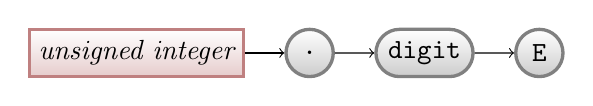
\begin{tikzpicture}[start chain,node distance=5mm, every node/.style={on chain,join}, every join/.style={->}]
    \node [nonterminal]  {unsigned integer};
    \node [terminal]     {.};
    \node [terminal]     {digit};
    \node [terminal]     {E};
  \end{tikzpicture}
\end{figure}
\end{document}